\documentclass{article} % For LaTeX2e
\usepackage{nips15submit_e,times}
\usepackage{hyperref}
\usepackage{url}
\usepackage{graphicx}
\graphicspath{{figures/}}
\usepackage{fixltx2e}
\usepackage[cmex10]{amsmath}
%\documentstyle[nips14submit_09,times,art10]{article} % For LaTeX 2.09


\title{Foreground/Background Segmentation with Probabilistic Graphical Models}


\author{
Weijian Zhou\thanks{Department of Electrical and Computer Engineering, University of Toronto, Toronto, ON, M5S 3G4} \\
997107018 \\
\texttt{keith.zhou@mail.utoronto.ca} \\
\And
ChenXing Zhao \thanks{Department of Electrical and Computer Engineering, University of Toronto, Toronto, ON, M5S 3G4} \\
995965139\\
\texttt{chenxing.zhao@mail.utoronto.ca} \\
\AND
Wenzhangzhi Guo\thanks{Department of Electrical and Computer Engineering, University of Toronto, Toronto, ON, M5S 3G4} \\
997573353 \\
\texttt{wenzhi.guo@mail.utoronto.ca} \\
}

% The \author macro works with any number of authors. There are two commands
% used to separate the names and addresses of multiple authors: \And and \AND.
%
% Using \And between authors leaves it to \LaTeX{} to determine where to break
% the lines. Using \AND forces a linebreak at that point. So, if \LaTeX{}
% puts 3 of 4 authors names on the first line, and the last on the second
% line, try using \AND instead of \And before the third author name.

\newcommand{\fix}{\marginpar{FIX}}
\newcommand{\new}{\marginpar{NEW}}

\nipsfinalcopy % Uncomment for camera-ready version

\begin{document}


\maketitle

\begin{abstract}
In this paper, we experiment with four different inference and learning models on an image segmentation problem. The goal of the project is to segment each image into foreground pixels and background pixels by finding the mask that cuts out the foreground image. The foreground and background objects in each image come from a known library. In this case, there are five different foreground objects and seven different background objects. The four inference algorithm we look at in this paper include iterated conditional modes (ICM), exact expectation-maximization (EM), Gibbs sampling EM, and variational (mean-field) EM. The basic idea of the four inference algorithms is to approximate the joint distribution of the visible and hidden variables with a \textit{Q}-distribution. Different inference algorithms put slightly different restrictions on the \textit{Q}-distribution. This \textit{Q}-distribution can be found by minimizing the free-energy (KL-divergent of the posterior distribution and the \textit{Q}-distribution). Based on our experimental result, exact EM achieved the best result, but it also took longer to run. ICM took very little computational time, but it returned the worst result. 
\end{abstract}

\section{Introduction}
\label{intro}
In recent years, there is increasing interest in solving machine learning problems with probabilistic graphical models. Probabilistic graphical models not only provide a simple way to visualize the interactions between different variables in a model, they also allow complex probabilistic computations to be expressed as graphical manipulations \cite{b1}. In a graphical model, two of the main issues we are trying to solve are inference (compute the expectation of certain nodes given some observed nodes) and learning (setting the parameters of the model given some data). In this paper, we are going to follow the approaches in \cite{b2} to compare four different inference and learning algorithms: iterated conditional modes (ICM), exact expectation-maximization (EM), Gibbs sampling EM, and variational (mean-field) EM. In order to compare the above four algorithms quantitatively, those four algorithms were tested against a simple image segmentation problem where we are trying to describe pictures as a composition of foreground and background objects, selected from a pre-defined library. Segmenting an image into foreground and background can be helpful to solve many other computer vision problems such as object classification \cite{b2}.

All four inference and learning algorithms mentioned above have been widely used in many different image segmentation problems. The basic idea is to approximate the joint distribution of the visible and hidden variables with a \textit{Q}-distribution. ICM is initially introduced by Besag in 1983 \cite{b3} and since then, the original algorithm and its variants have been applied to many different image segmentation problems \cite{b4} \cite{b5} \cite{b6}. In general, ICM iterates between finding the optimal value of each hidden variable \textit{h}\textsubscript{\textit{i}} and finding the optimal values for the model parameters \cite{b2}. On the other hand, the three EM algorithms accounts for uncertainty in the random variables in the update rules \cite{b2}. For exact EM, there is no restrictions on the \textit{Q}-distributions. For the Gibbs Sampling EM, we use sampling method to update the hidden variables in the E-step. Lastly, mean-field EM assumes the \textit{Q}-distribution can be fully factorized. EM algorithms are also widely used for image segmentation problems \cite{b7} \cite{b8} \cite{b9} \cite{b10}.

\section{Algorithms}
\label{alog}
\subsection{Data generation}
\label{data_gen}
A training image used in this paper is generated using the following procedure:
\begin{itemize}

\item Randomly select a foreground image. Each foreground image has a fixed mask which specifies the location of the foreground image within the background image.

\item Randomly select a background image.

\item Combine the foreground image and background image with the cut-out mask.

\item Add Gaussian noise. The Gaussian noise is added to model sensor noise and change in illumination so that we can have more data available for training. 
\end{itemize}

The training image is the only data that is shown to our model in the training process. A graphical illustration of the above procedures can be seen in Fig~\ref{fig:data_generation}.

\begin{figure}[h]
\begin{center}
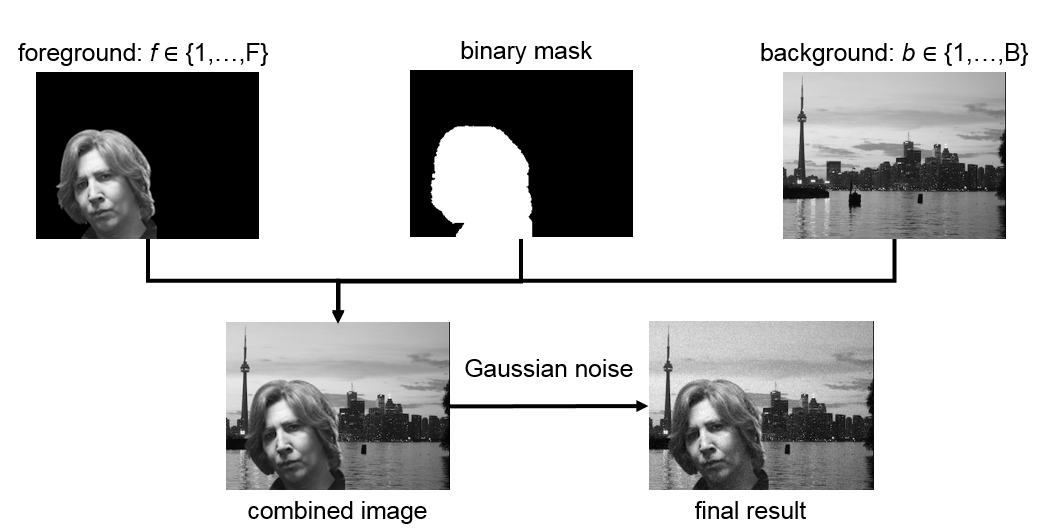
\includegraphics[width=1\textwidth]{data_generation}
\end{center}
\caption{Overview of data generation}
\label{fig:data_generation}
\end{figure}

\subsection{Model}
\label{model}
In this project, we are using an occlusion model to describe each image generated in \ref{data_gen}, where the foreground object and background object in each image come from the same library with \textit{J} objects. If we assume each image has \textit{K} pixels, then we can denote the pixel intensity in an image by \textit{z}\textsubscript{\textit{1}}, \ldots , \textit{z}\textsubscript{\textit{K}}. The probability of choosing \textit{f}\textsuperscript{\textit{th}} foreground object is \textit{P(f)}. Then depending on the foreground object, a binary mask is constructed \textit{m} = (\textit{m}\textsubscript{\textit{1}}, \ldots, \textit{m}\textsubscript{\textit{K}}). \textit{m}\textsubscript{\textit{i}} is either 0 (pixel \textit{z}\textsubscript{\textit{i}} is a background pixel) or 1 (pixel \textit{z}\textsubscript{\textit{i}} is a foreground pixel). The binary mask must cut out the foreground object, but given the foreground object, the mask RVs are independent. Similarly, the probability of choosing \textit{b}\textsuperscript{\textit{th}} background object is \textit{P(b)}. Lastly, when given the mask, the foreground object class and background object class, the intensities of the pixels in an image are independent. Therefore, the joint distribution of the model can be written as:
\begin{equation}
P(z,m,f,b) = P(b)P(f)\Bigg( \prod_{i=1}^KP(m_{i}|f)\Bigg)\Bigg( \prod_{i=1}^KP(z_{i}|m_{i},f,b)\Bigg)
\label{eq:eq1}
\end{equation}

Since the mask RVs (\textit{m}\textsubscript{\textit{i}}) are binary, the last term in equation~\ref{eq:eq1} can be factorized. When \textit{m}\textsubscript{\textit{i}} = 0, the pixel intensity (\textit{z}\textsubscript{\textit{i}}) only depends on the background object index \textit{b}, whereas when \textit{m}\textsubscript{\textit{i}} = 1, \textit{z}\textsubscript{\textit{i}} only depends on the foreground object index \textit{f}. Therefore, equation~\ref{eq:eq1} can be re-written as:
\begin{equation}
P(z,m,f,b) = P(b)P(f)\Bigg( \prod_{i=1}^KP(m_{i}|f)\Bigg)\Bigg( \prod_{i=1}^KP(z_{i}|f)^{m_{i}}\Bigg)\Bigg( \prod_{i=1}^KP(z_{i}|b)^{1-m_{i}}\Bigg)
\label{eq:eq2}
\end{equation}

To reduce the computation complexity, it is often useful to parametrize the model. In this case, we assume the pixel intensities in each image follows a Gaussian distribution, where given a foreground or background object index \textit{k}, the pixel intensity \textit{z}\textsubscript{\textit{i}} equals to \textit{$\mu$}\textsubscript{\textit{ki}} plus zero-mean Gaussian noise with a variance of \textit{$\psi$}\textsubscript{\textit{ki}}. We also denote the probability of class \textit{k} by \textit{$\pi$}\textsubscript{\textit{k}}. Lastly, we denote the probability of \textit{m}\textsubscript{\textit{i}} = 1, given the foreground class is \textit{f} by \textit{$\alpha$}\textsubscript{\textit{fi}}. Using this parametrization, equation~\ref{eq:eq2} can be written as:
\begin{equation}
P(z,m,f,b) = \pi_{b} \pi_{f} \Bigg( \prod_{i=1}^K {(\alpha_{fi})}^{m_{i}} {(1-\alpha_{fi})}^{1-m_{i}} \mathcal{N}(z_i;\mu_{fi},\psi_{fi})^{m_{i}}\mathcal{N}(z_i;\mu_{bi},\psi_{bi})^{1-m_{i}} \Bigg)
\label{eq:eq3}
\end{equation}

where $\mathcal{N}$ represents the Gaussian distribution. 

\subsection{Finding model parameters by minimizing the free energy}
\label{free_energy}
The model parameters are found based on each training image. In each training image, we can group the variables into hidden RVs, visible RVs and parameters. The visible RVs in this case are the pixel intensities: \textit{v}\textsuperscript{\textit{(t)}} = \textit{z}\textsuperscript{\textit{(t)}}. The hidden RVs are \textit{h}\textsuperscript{\textit{(t)}} = (\textit{f}\textsuperscript{\textit{(t)}}, \textit{b}\textsuperscript{\textit{(t)}}, \textit{m}\textsuperscript{\textit{(t)}}). The model parameters are \textit{$\theta$} = (\textit{$\mu$}, \textit{$\psi$}, \textit{$\pi$}, \textit{$\alpha$}). Then the joint distribution of the visible and hidden RVs can be written as:
\begin{equation}
P(h,v) = P(\theta) \prod_{t=1}^TP\Big(h^{(t)}, v^{(t)}|\theta\Big) 
\label{eq:eq4}
\end{equation}
where (t) represents the index of the training cases.

Usually, it is very difficult to find the posterior distribution P(\textit{h}\textbar\textit{v}) directly since the calculation for the partition function is intractable. Therefore, we often use approximate inference techniques instead. The basic idea of those techniques is that we are trying to use a simpler \textit{Q}-distribution, Q(\textit{h}), to approximate the true posterior distribution P(\textit{h}\textbar\textit{v}). The free energy is a measurement of similarity between the true posterior distribution and the \textit{Q}-distribution we have currently. The free energy is defined as:
\begin{equation} \label{eq:eq5}
\begin{split}
F(Q,P) &= KL(Q,P) - \ln P(v) \\
& = \int_{h} Q(h)\ln \frac{Q(h)}{P(h|v)} - \int_{h} Q(h)\ln P(v) \\
& = \int_{h} Q(h)\ln \frac{Q(h)}{P(h,v)} 
\end{split}
\end{equation}
where KL(\textit{Q},\textit{P}) is the KL-divergent between the \textit{Q}-distribution and the posterior distribution P(\textit{h}\textbar\textit{v}). The term ln P(\textit{v}) is added to make the calculation tractable (since we do not have a tractable form of P(\textit{h}\textbar\textit{v})), but it does not have a direct impact final solution for the \textit{Q}-distribution (since P(\textit{v}) does not depend on the \textit{Q}-distribution). Since the KL divergence is a similarity measure of two distributions, minimizing the free energy F(\textit{Q},\textit{P})) makes the \textit{Q}-distribution more similar to the posterior distribution P(\textit{h}\textbar\textit{v}). Therefore, the goal of the inference problem is to search through the space to find Q(\textit{h}) that resembles the true posterior distribution closely. 

If we assume the training data is i.i.d, we can de-couple the free energy so that we have one term for each training case. In this case, we can substitute equation~\ref{eq:eq4} into equation~\ref{eq:eq5} and obtain:
\begin{equation}
F(Q,P) = \int_{h} Q(h)\ln Q(h) - \int_{\theta} Q(\theta)\ln P(\theta) - \sum_{t=1}^T \int_{h^{(t)},\theta}Q(h^{(t)},\theta)\ln P\Big(h^{(t)}, v^{(t)}|\theta\Big) 
\label{eq:eq6}
\end{equation}


\subsection{Iterated Conditional Modes (ICM)}
\label{icm}
The ICM algorithm alternates between updating the hidden variables and the model parameters. In the ICM update procedure, we are only considering local information. We update one variable/parameter at a time by setting it to its Maximum a posterior (MAP) value while holding other variables/parameters constant. Since we are using the MAP estimation where there is a hard-assignment for each pixel (it either belongs to the foreground or the background class), the \textit{Q}-distribution is a product of delta functions:
\begin{equation} \label{eq:eq7}
\begin{split}
Q = &\Bigg( \prod_{k}\delta(\pi_k-\hat{\pi}_k) \Bigg) \Bigg( \prod_{k,i}\delta(\mu_{ki}-\hat{\mu}_{ki}) \Bigg)\Bigg( \prod_{k,i}\delta(\psi_{ki}-\hat{\psi}_{ki}) \Bigg)\Bigg( \prod_{k,i}\delta(\alpha_{ki}-\hat{\alpha}_{ki}) \Bigg) \\
&\Bigg( \prod_{t}\Big[b^{(t)} = \hat{b}^{(t)}\Big] \Bigg)\Bigg( \prod_{t}\Big[f^{(t)} = \hat{f}^{(t)}\Big] \Bigg)\Bigg( \prod_{t}\prod_{i}\Big[m_i^{(t)} = \hat{m}_i^{(t)}\Big] \Bigg)
\end{split}
\end{equation}
Substituting equation~\ref{eq:eq7} and ~\ref{eq:eq3} into equation~\ref{eq:eq6}, taking the derivative with respect to each parameter/ variable and setting the derivative to zero, we can find the update rule for the ICM model as follows (Repeat until convergence):

\textbf{E-step (hidden variable updates)}

for t = 1, \ldots , T:
\begin{align*} 
&f \leftarrow \text{argmax}_{f}\Bigg(\pi_f \prod_{i=1}^K\Big({(\alpha_{fi})}^{m_{i}} {(1-\alpha_{fi})}^{1-m_{i}}\mathcal{N}(z_i;\mu_{fi},\psi_{fi})^{m_{i}}\Big)\Bigg)\\
&\text{for i = 1, \ldots , K: } \\
& \text{ }\text{ }\text{ }\text{ }\text{ }m_i \leftarrow \text{argmax}_{m_i}=\begin{cases}
\alpha_{fi}\mathcal{N}(z_i;\mu_{fi},\psi_{fi}), & \text{if $m_i = 1$}\\
(1-\alpha_{fi})\mathcal{N}(z_i;\mu_{bi},\psi_{bi}), & \text{if $m_i = 0$}
\end{cases} \\
&b \leftarrow \text{argmax}_{b}\Bigg(\pi_b \prod_{i=1}^K \mathcal{N}(z_i;\mu_{bi},\psi_{bi})^{1-m_{i}}\Bigg)
\end{align*} 

\textbf{M-step (model parameter updates)}

For j = 1, \ldots , J: 
\begin{equation*}
\pi_j \leftarrow \frac{1}{2T}\sum_{t=1}^T([f^{(t)} = j] + [b^{(t)} = j])
\end{equation*}
For j = 1, \ldots , J: For i = 1, \ldots , K: 
\begin{align*} 
&\alpha_{ji} \leftarrow \frac{\sum_{t=1}^T [f^{(t)} = j]m_i^{(t)}}{\sum_{t=1}^T [f^{(t)} = j]} \text{ }\text{ }\text{ }\text{ }\text{ }\mu_{ji} \leftarrow \frac{\sum_{t=1}^T [f^{(t)} = j \text{ or } b^{(t)} = j ]z_i^{(t)}}{\sum_{t=1}^T [f^{(t)} = j \text{ or } b^{(t)} = j]} \\
&\psi_{ji} \leftarrow \frac{\sum_{t=1}^T [f^{(t)} = j \text{ or } b^{(t)} = j ](z_i^{(t)}-\mu_{ji})^2}{\sum_{t=1}^T [f^{(t)} = j \text{ or } b^{(t)} = j]} 
\end{align*} 

The ICM algorithm is really easy to implement, but it can get stuck at local optima very easily. Thus, this algorithm does not work well in many cases in practice.

\subsection{Exact Expectation-Maximization (EM)}
\label{exact_em}

Unlike ICM, the EM algorithm takes into account for uncertainty in the RVs in the update process. The \textit{Q}-distribution for the i.i.d training cases can be written as:
\begin{equation}
Q(h) = \delta(\theta-\hat{\theta})\prod_{t=1}^TQ(h^{(t)})
\label{eq:eq8}
\end{equation}

Substituting equation~\ref{eq:eq8} into equation~\ref{eq:eq6}, taking the derivative with respect to each parameter/ variable and setting the derivative to zero, we can find the update rule for exact EM as follows:

\textbf{E-step}

for t = 1, \ldots , T: 
\begin{align*} 
&Q(b,f) \leftarrow c_2\pi_b\pi_f\prod_{i=1}^K\Bigg(\alpha_{fi}\mathcal{N}(z_i;\mu_{fi},\psi_{fi})+ (1-\alpha_{fi})\mathcal{N}(z_i;\mu_{bi},\psi_{bi}) \Bigg) \\
&Q(b) \leftarrow \sum_{f} Q(b,f) \text{ }\text{ }\text{ }\text{ }\text{ }\text{ }\text{ }\text{ }\text{ }\text{ }Q(f) \leftarrow \sum_{b} Q(b,f) \\\\
&\text{for i = 1, \ldots , K: } \\
&\text{ }\text{ }\text{ }\text{ }\text{ }Q(m_i = 1|b,f) \leftarrow c_1\alpha_{fi}\mathcal{N}(z_i;\mu_{fi},\psi_{fi})\text{ }\text{ }\text{ }\text{ }\text{ }Q(m_i = 0|b,f) \leftarrow c_1(1-\alpha_{fi})\mathcal{N}(z_i;\mu_{bi},\psi_{bi})\\
&\text{for i = 1, \ldots , K: } \\
&\text{ }\text{ }\text{ }\text{ }\text{ }Q(m_i,b) \leftarrow \sum_{f}Q(m_i|b,f) Q(b,f)\text{ }\text{ }\text{ }\text{ }\text{ }Q(m_i,f) \leftarrow \sum_{b}Q(m_i|b,f) Q(b,f)\\
\end{align*} 

\textbf{M-step}

For j = 1, \ldots , J: 
\begin{equation*}
\pi_j \leftarrow \frac{1}{2T}\sum_{t=1}^T\Bigg(Q(f^{(t)} = j) + Q(b^{(t)} = j)\Bigg)
\end{equation*}
For j = 1, \ldots , J:  For i = 1, \ldots , K: 
\begin{align*} 
&\alpha_{ji} \leftarrow \frac{\sum_{t=1}^T Q(m_i^{(t)}=1,f^{(t)} = j)}{\sum_{t=1}^TQ(f^{(t)} = j)} \\
&\mu_{ji} \leftarrow \frac{\sum_{t=1}^T\Big(Q(m_i^{(t)}=1,f^{(t)} = j) + Q(m_i^{(t)}=0,b^{(t)} = j)\Big)z_i^{(t)}}{\sum_{t=1}^T \Big(Q(m_i^{(t)}=1,f^{(t)} = j) + Q(m_i^{(t)}=0,b^{(t)} = j)\Big)} \\
&\psi_{ji} \leftarrow \frac{\sum_{t=1}^T\Big(Q(m_i^{(t)}=1,f^{(t)} = j) + Q(m_i^{(t)}=0,b^{(t)} = j)\Big)(z_i^{(t)}-\mu_{ji})^2}{\sum_{t=1}^T \Big(Q(m_i^{(t)}=1,f^{(t)} = j) + Q(m_i^{(t)}=0,b^{(t)} = j)\Big)} \\
\end{align*} 

\subsection{Gibbs Sampling EM}
\label{gibbs_em}
Gibbs sampling EM is very similar to ICM except it uses Gibbs sampling to update the hidden variables in the E-step. Since this sampling approach is a stochastic process, it helps the algorithm to jump out from local optima in certain cases and thus improving the overall performance of the algorithm. The M-step in this case is the same as ICM, but the E-step is modified to:

\textbf{E-step}

for t = 1, \ldots , T:
\begin{align*} 
&f \leftarrow \text{sample}_{f}\Bigg(\pi_f \prod_{i=1}^K \Big({\alpha_{fi}\mathcal{N}(z_i;\mu_{fi},\psi_{fi})}\Big)^{m_{i}} {(1-\alpha_{fi})}^{1-m_{i}}\Bigg)\\
&\text{for i = 1, \ldots , K: } \\
& \text{ }\text{ }\text{ }\text{ }\text{ }m_i \leftarrow \text{sample}_{m_i}\begin{cases}
\alpha_{fi}\mathcal{N}(z_i;\mu_{fi},\psi_{fi}), & \text{if $m_i = 1$}\\
(1-\alpha_{fi})\mathcal{N}(z_i;\mu_{bi},\psi_{bi}), & \text{if $m_i = 0$}
\end{cases} \\
&b \leftarrow \text{sample}_{b}\Bigg(\pi_b \prod_{i=1}^K \mathcal{N}(z_i;\mu_{bi},\psi_{bi})^{1-m_{i}}\Bigg)
\end{align*} 

\subsection{Variational (Mean field) EM}
\label{variational_em}

In the variational EM, we assume the hidden variables in the \textit{Q}-distribution factorizes completely into \textit{L} distributions, where \textit{L} is the number of hidden RVs:

\begin{equation}
Q(h) = \prod_{i=1}^LQ(h_i) 
\label{eq:eq9}
\end{equation}

In this case, the E-step can be simplified to:

\textbf{E-step}

for t = 1, \ldots , T:
\begin{align*} 
&Q(f) \leftarrow c_3\pi_f\prod_{i=1}^K\Bigg(\Big(\alpha_{fi}\mathcal{N}(z_i;\mu_{fi},\psi_{fi})\Big)^{Q(m_i=1)} (1-\alpha_{fi})^{Q(m_i=0)} \Bigg) \\
&\text{for i = 1, \ldots , K: } \\
&\text{ }\text{ }\text{ }\text{ }\text{ }Q(m_i = 1) \leftarrow c_1\prod_{f}\Bigg(\alpha_{fi}\mathcal{N}(z_i;\mu_{fi},\psi_{fi})\Bigg)^{Q(f)}\\
&\text{ }\text{ }\text{ }\text{ }\text{ }Q(m_i = 0) \leftarrow c_1\Bigg(\prod_{f}(1-\alpha_{fi})^{Q(f)}\Bigg)\Bigg(\prod_{b}\mathcal{N}(z_i;\mu_{bi},\psi_{bi})^{Q(b)}\Bigg)\\
&Q(b) \leftarrow c_2\pi_b\prod_{i=1}^K\mathcal{N}(z_i;\mu_{bi},\psi_{bi})^{Q(m_i=0)}
\end{align*} 

The M-step is the same as in the exact EM except the joint distributions can be written as two marginal distributions (due to independence) as the following:

\begin{align*} 
&Q(m_i^{(t)},f^{(t)})  = Q(m_i^{(t)}) Q(f^{(t)}) \\
&Q(m_i^{(t)},b^{(t)})  = Q(m_i^{(t)}) Q(b^{(t)}) 
\end{align*} 

\subsection{Other Inference Algorithms}
Structured variational EM and sum-product EM can also be used to solve the image segmentation problem described in this paper. However, we did not have time to implement and test them due to time constraint. Unlike mean-field approximation, the structured variational EM takes into account some dependencies between the hidden RVs. In general, if more dependencies are included in the model, we will have more exact inference, but the computational complexity also increases. The sum-product algorithm performs inference by message passing. If the graphical model is a tree, all the posterior marginal distributions will be exact once we have passed the messages from the leaves to the root and then from the root back to the leaves. However, in out case, the graphical model constructed for this problem has cycles. The messages need to be passed through the model several times until convergence. The details of the update equations for these two models can be found in \cite{b2}.

\section{Experimental Results}
\label{result}
\subsection{Data set}
\label{data_set}
The data set used for this project can be seen in Fig~\ref{fig:data_set}. There were five foreground objects and seven background objects used to create the training images. A total of 350 images (10 noisy images of each combination of the foreground and background images) were used as training images for this project. Each inference algorithm was run 10 times with different random initializations and the result with the highest likelihood was reported.

\begin{figure}[h]
\begin{center}
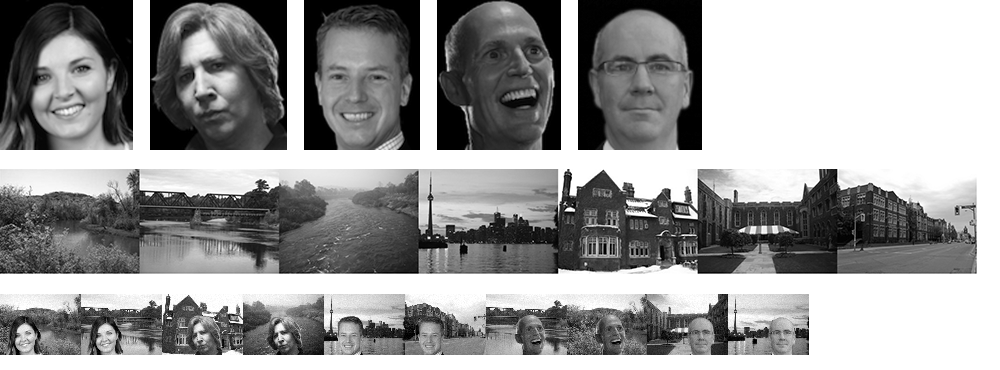
\includegraphics[width=1\textwidth]{data_set}
\end{center}
\caption{Data set used this project. first row: foreground images. second row: background images (resized). third row: example of training images}
\label{fig:data_set}
\end{figure}

\subsection{Parameter Learning Results}
\label{parameter_result}
A sample of the learned parameters for each inference algorithm can be seen in Fig~\ref{fig:model_com}. The model assumes there are 14 clusters (2 more than the sum of total number of foreground and background objects in the library) to give the model more flexibility. For the ICM, we can see that the mask probabilities are mostly random. The combination of the mask probabilities with the mean image (second column) does not produce any sensible foreground image. Thus, the ICM does not produce very good segmentation results. This is mainly due to the fact that ICM gets stuck at local optima easily. Once it gets stuck, there is no way to get out of it. For the exact EM, the performance is much better. The model learned accurate mask for class 1, 6, and 7 and partially accurate mask for class 2 and 3. Since there are 5 different foreground objects in the library, we expect that there are 5 classes with clean mask (classes with clean masks are foreground images, and the rest are background images). Thus, the result of the exact EM is fairly close to what we expected. For the mean-field EM, class 9 and class 13 produces mask that is roughly in the correct location (with some noise). Therefore, the performance of mean-field EM is worse than the exact EM. The mean-field EM simplifies the exact EM model by assuming the \textit{Q}-distribution completely factorizes. This assumption ignores dependencies between hidden RVs, causing it to perform worse than the exact EM. However, in more complicated problems, this simplification can greatly reduce the computational complexity. Lastly, for Gibbs sampling EM, class 1 and class 5 each produces a very crude estimation of the mask. The masks produced in those two classes are not very accurate in terms of location and are very blurry. However, this result is much better than the result produced by ICM. The reason for this is performing Gibbs takes uncertainties into account, which helps the model to get out of local optima it encounters in certain cases (whereas in ICM, the hidden RVs are updated based on their MAP value, so the model cannot escape those local optima). Therefore, based on the plot in Fig~\ref{fig:model_com}, we can rank the performance of the four models as follows (from best to worst): exact EM, mean-field EM, Gibbs sampling EM, and ICM.

Comparing to the result in \cite{b2}, a similar trend is observed. ICM failed to find any sensible classes. The exact EM performs the best where it was able to successfully infer all foreground and background classes correctly. The mean-filed was able to infer the foreground and background classes correctly, except sometimes there are cutting holes in the learned mask. However, the results obtained in \cite{b2} for the exact EM and mean-field EM are better than what we were able to get in this project. The possible explanations for this difference could be because of the different dataset that was used and the differences in the implementation details.

\begin{figure}[h]
\begin{center}
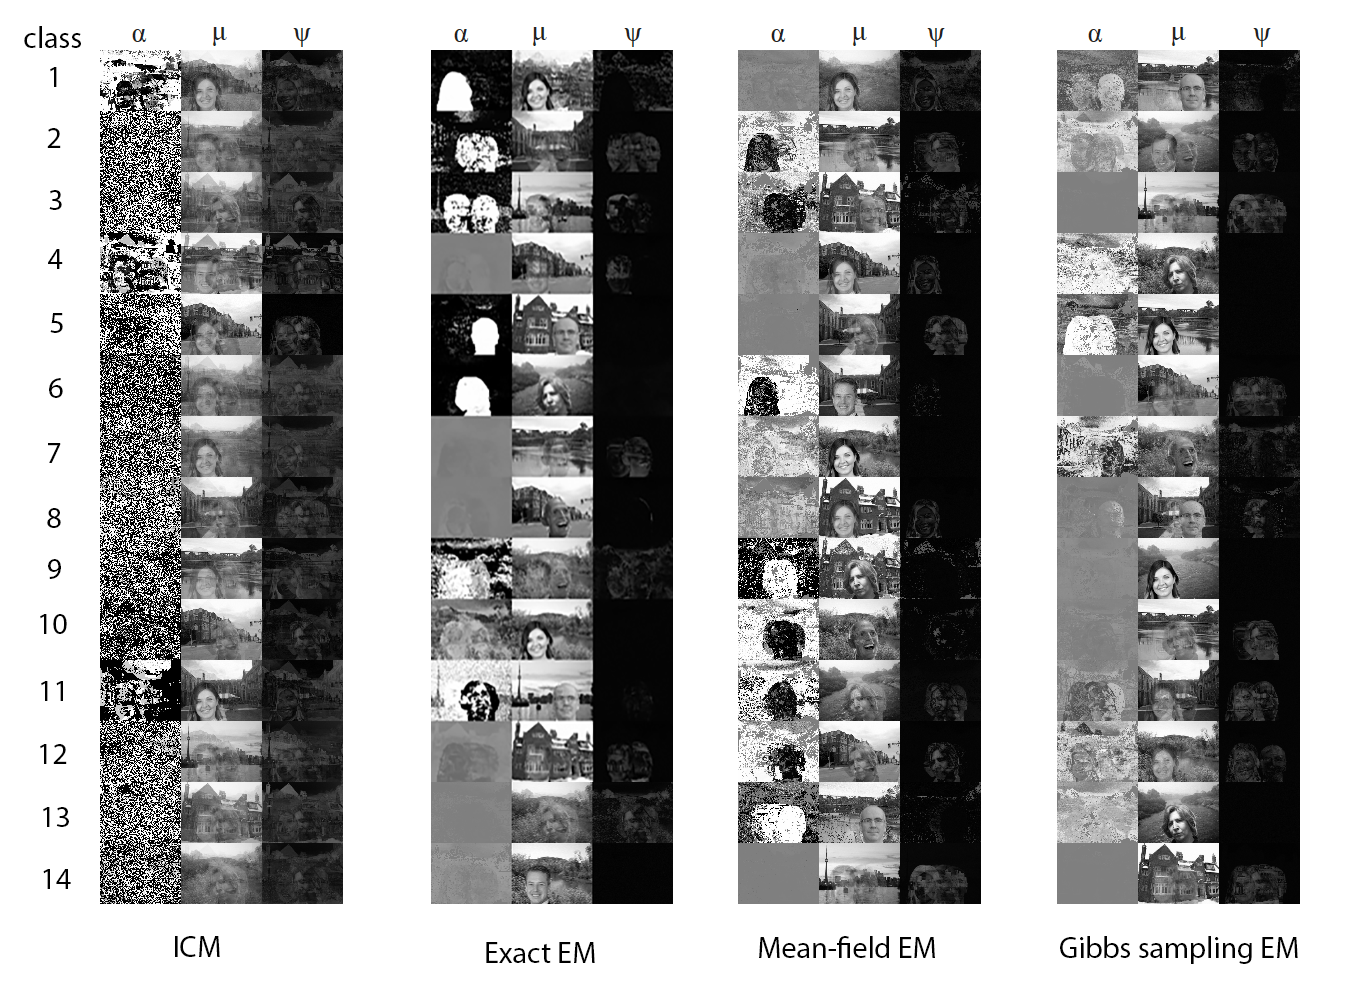
\includegraphics[width=1\textwidth]{final_plot1}
\end{center}
\caption{Comparison of the learned parameters using four different inference algorithms. \textit{$\alpha$} represents the mask probability for each pixel (white represents a high probability), \textit{$\mu$} represents the pixel means and \textit{$\psi$} represents the pixel variances}
\label{fig:model_com}
\end{figure}

\subsection{Free Energy Results}
\label{free_energy_result}
The free energy across different iterations can be seen in Fig~\ref{fig:free_energy}. Since the free energy is a measure of the similarity between the \textit{Q}-distribution and the true posterior distribution, a well-trained model should have low free energy. For all four inference algorithms, the free energy decreases very quickly in the first 5 iterations, then converges to a relatively stable value afterwards. The initial drastic change in the free energy is due to the fact that all the variables were initialized randomly, so most of them are far from optimal values (causing the system to have a huge free energy initially). Thus, those variables need to be changed by a large amount initially to get closer to their optimal values (as the \textit{Q}-distribution gets closer to the true posterior distribution), causing a big decrease in the free energy. After 5 iterations, the hidden variables and parameters are at their optimal values mostly, so most of them will not change across iterations or only very tiny adjustments are made. As a result, the free energy stays relatively stable at this point. 

The free energy of ICM converges to its steady state value the quickest while the Gibbs sampling EM takes the longest to converge. The reason for this is ICM algorithm quickly gets stuck at local optima where the Gibbs sampling EM tries to get out of local optima by taking uncertainties into account.

There are some oscillations seen in the free energy curve for Gibbs sampling EM. Those oscillations are cases where the hidden RVs were not updated based on their MAP value by taking the uncertainties into account. Even though taking uncertainties into account makes the free energy increases sometimes, those uncertainties enable the inference algorithm to escape from local optima, which lead to a better solution. However, the free energy of Gibbs sampling EM is still lower than that of ICM. 

The trend seen in the free energy plot matches the trend seen in \ref{parameter_result}. The best performing model (exact EM) has the lowest free energy while the worst performing model (ICM) has the highest free energy after the model converges. The trend seen in our free energy plot matches the free energy plot in \cite{b2}. However, the exact range of the free energy curve is not the same. This is due to the fact that the training images in our case has different dimensions than the ones used in \cite{b2} and we used 350 training images instead of 300 training images. 
\begin{figure}[h]
\begin{center}
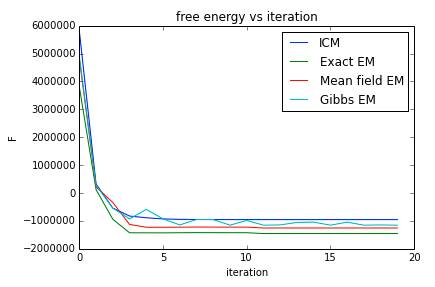
\includegraphics[width=1\textwidth]{free_energy}
\end{center}
\caption{Comparison of the free energy for the four inference algorithms across iterations}
\label{fig:free_energy}
\end{figure}

\subsection{Runtime Analysis}
\label{runtime}
The runtime of each algorithm is highly dependent on the implementation and hardware. For this project, the run time for each algorithm can be seen in Table~\ref{tab:runtime}. The ICM has the smallest runtime while exact EM has the largest runtime. This result matches the complexity analysis in \cite{b2} where the exact inference has the highest complexity and ICM has the lowest complexity. However, even though Gibbs sampling and ICM has the same complexity in \cite{b2}, the runtime of Gibbs sampling is larger than that of ICM in the implementation. The reason for this is it takes longer to collect samples in the Gibbs sampling EM than just using the MAP value.

\begin{table}[h]
\centering
\caption{Runtime Comparison}
\label{tab:runtime}
\begin{tabular}{|c|c|c|c|c|}
\hline
& ICM & Exact EM & Mean-field EM & Gibbs Sampling EM \\ \hline
runtime per iteration (sec) & 4.09 & 32.34 & 20.51 & 9.26 \\ \hline
\end{tabular}
\end{table}

\section{Conclusions}
\label{conclusion}
In this project, we looked at four different inference algorithms (ICM, exact EM, mean-filed EM, and Gibbs sampling EM) and compared their performance with a simple image segmentation problem. Exact EM has the best performance, but it also has the largest runtime. Mean-filed EM reduces the complexity of exact EM by assuming the \textit{Q}-distribution can be completely factorized. This assumption reduces the runtime, but also worsen the performance a little bit. ICM has the fastest runtime, but it has very poor performance. The performance of ICM can be improved by taking uncertainty into account, which leads to the Gibbs sampling EM.

In the future, we plan to implement structural variational inference and sum-product EM as well and test their performance on this problem. Additionally, we plan to apply those inference algorithms to other image segmentation problems.

\small{
\begin{thebibliography}{1}

\bibitem{b1} Bishop, C.M., ``Graphical Models," in \textit{Pattern recognition and machine learning,} New York, NY, USA: Springer Science+Business Media, LLC, 2006, ch. 8, pp. 359-360.

\bibitem{b2} Frey, B.J. and Jojic, N., ``A comparison of algorithms for inference and learning in probabilistic graphical models," \textit{IEEE Trans. Pattern Anal. Mach. Intell.,} vol. 27, no. 9, pp. 1392–1416, Sept. 2005.

\bibitem{b3} Besag, J.E. ``Discussion of paper by P. Swiller," \textit{Bull. Inr. Stafisr. Inst.,} vol. 50, no. 3, pp. 422-425, 1983.

\bibitem{b4} Loog, M. and van Ginneken, B., ``Supervised segmentation by iterated contextual pixel classification,” \textit{Image Signal Process., ser. Proc. 16th Int. Conf. Pattern Recognition (ICPR 2002),} pp. 925–928, 2002.

\bibitem{b5} Owen, A., ``Image segmentation via iterated conditional expectations," Department of Statistics, Stanford University, Stanford, CA, Tech. Rep. 18 (94305-4065), June, 1989.

\bibitem{b6} Chen, C.W.; Luo, J.B. and Parker, K.J., ``Image segmentation via adaptive K-mean clustering and knowledge-based morphological operations with biomedical applications,” \textit{IEEE Trans. Imag. Processing,} vol. 7, pp. 1673–1683, Dec. 1998.

\bibitem{b7} Gu, D.B.and Sun, J.X., ``EM image segmentation algorithm based on an inhomogeneous hidden MRF model,” \textit{IEEE Proc. Vision, Image and Signal Processing,} vol. 152, Issue 2, pp. 184 – 190, April 2005.

\bibitem{b8} Geman, S. and Geman, D., ``Stochastic Relaxation, Gibbs Distribution and the Bayesian Restoration of Images,” \textit{IEEE Trans. Pattern Anal. Mach. Intell.,} vol. 6, pp. 721-741, 1984.

\bibitem{b9} Zhou, Y.; Gong, Y. and Tao, H. ``Background segmentation using spatial-temporal multi-resolution MRF,” \textit{Proc. 7th IEEE Workshop (WACV/MOTIONS '05),} vol. 1, pp. 8–13, Jan. 2005.

\bibitem{b10} Cho, W.-H.; Kim, S.-H.; Park, S.-Y. and Park, J.-H., ``Mean field annealing EM for image segmentation," \textit{Proc. 2000 Int’l Conf. on Image Processing,} vol. 3, pp. 568-571, Sep. 2000.
  \end{thebibliography}
}

\end{document}



